\section{Margarita Kitaeva}
\label{sec:Margarita Kitaeva}

%\parindet=1cm
This is a picture from a really cool concert (see Figure~\ref{fig:concert} on page \pageref{fig:concert}).

\begin{figure}[htbp]
    \centering
    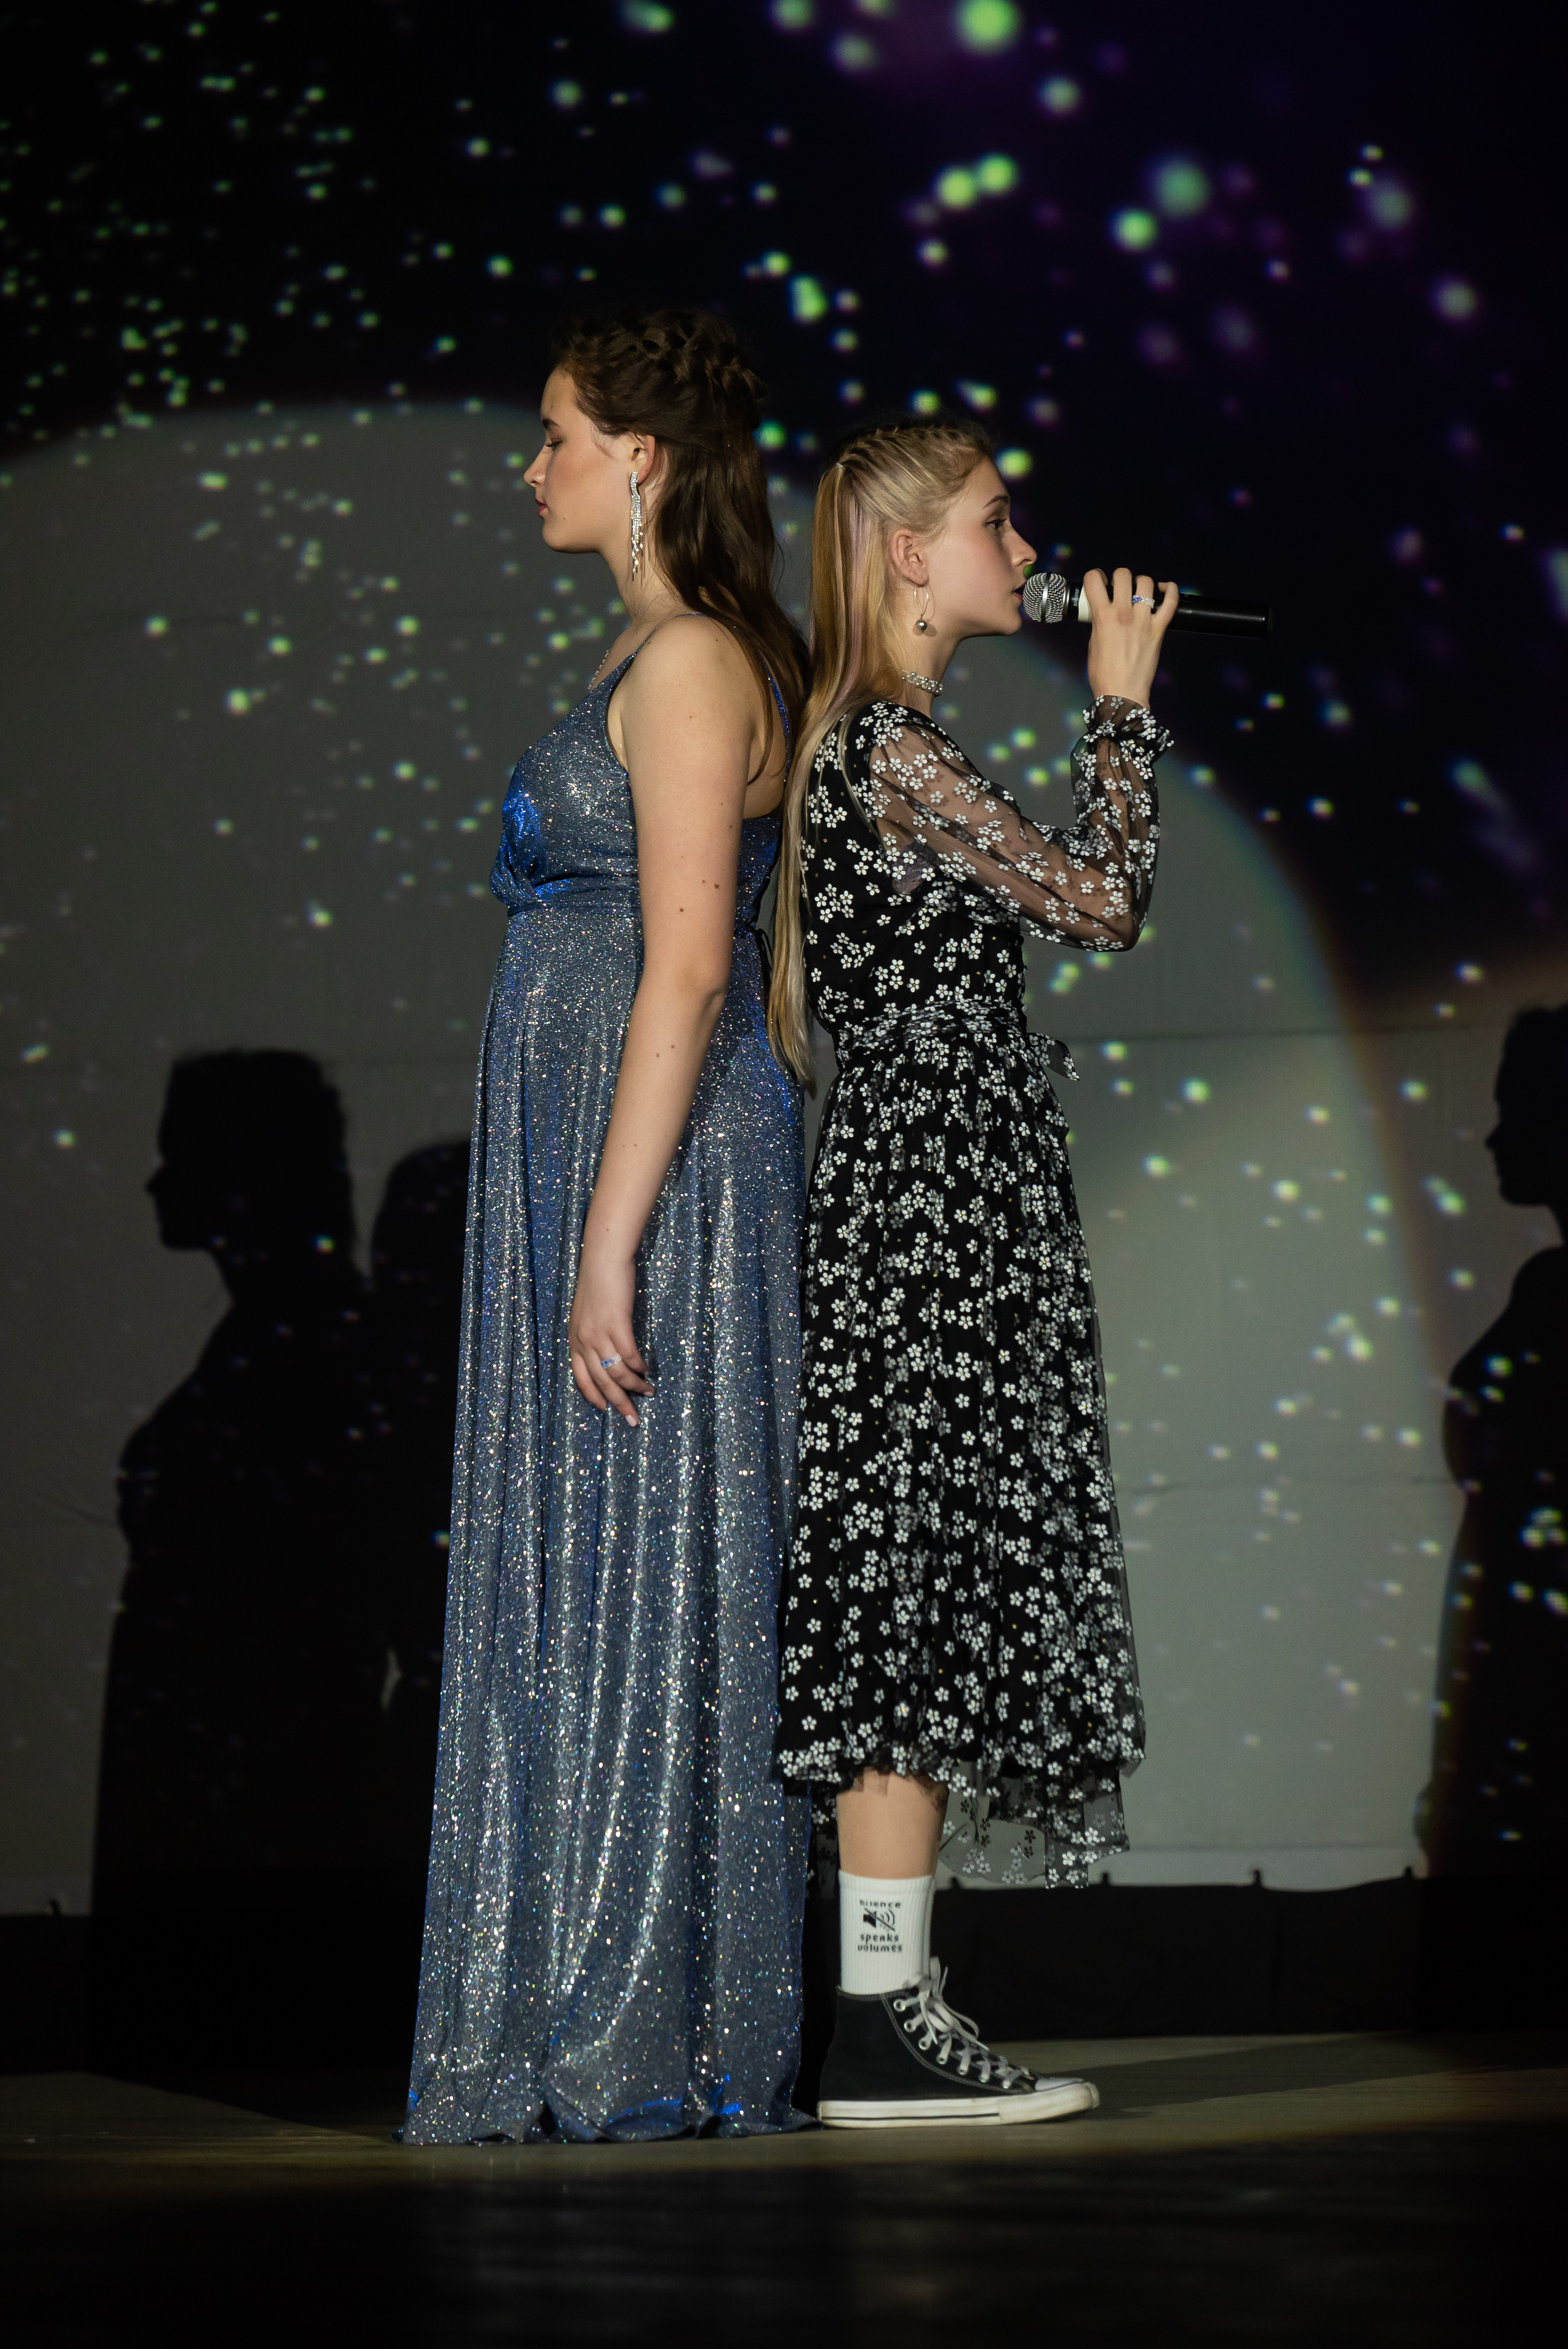
\includegraphics[width=0.5\textwidth]{pictures/concert.JPG}
    \caption{09.06.2023}
    \label{fig:concert}
\end{figure}

Table~\ref{sec:Margarita Kitaeva} on page \pageref{sec:Margarita Kitaeva} represents dates of birth of some people.
\begin{table}[htbp]
\centering
\begin{tabular}{|l|l|l|l|}
\hline
Name   & Day & Months & Year \\ \hline
Margo  & 21  & 02     & 2006 \\ \hline
Liza   & 11  & 09     & 2007 \\ \hline
Julia  & 12  & 12     & 2006 \\ \hline
Ilya   & 5   & 12     & 2006 \\ \hline
Maksim & 23  & 09     & 2006 \\ \hline
\end{tabular}
\label{tab:birthdays}
\caption{Here you can see some dates of birth}
\end{table}

Here is a formula of the magnetic field of an arbitrary flat contour: \[B = \frac{\mu I}{4\pi }\int_{\varphi _1}^{\varphi _2} \frac{d\varphi}{r(\varphi)}\]

And here is a formula of the magnetic field of an infinite wire:
$ B = \frac{\mu I}{2\pi R} $
    \begin{flushleft}    
    \begingroup
    \centering
    \title{\textbf{\Large Thirteen Reasons Why}}
    
    \endgroup
    \vspace{0.1cm}

    \setlength{\parindent}{1em}
    \underline{\textbf{13 Reasons Why}} is an American teen drama television series developed for \textit{Netflix} by Brian Yorkey and based on the 2007 novel \emph{"Thirteen Reasons Why" by author Jay Asher}. The series revolves around high school student Clay Jensen (Dylan Minnette) and the aftermath of the suicide of fellow student Hannah Baker (Katherine Langford). Before her death, she leaves behind a box of cassette tapes in which she details the reasons why she chose to end her life as well as the people she believes are responsible for her death. \par
    There are 4 seasons there and each season \emph{except 4th} consists of 13 series \emph{(4th consists of 10 series)}. This serial is really exciting and worth seeing. You can find some really interesting qoutes there. One of my favourites is \underline{this one}:
    
    \begingroup 
    \centering
    \textit{I guess that's the point of it all. No one knows for certain how much impact they have on the lives of other people. Oftentimes, we have no clue. Yet, we push it just the same.}
    
    \endgroup
 \end{flushleft}


\textbf{\large Here are some actors, who played main characters:}
\begin{itemize}
    \item Dylan Minnette as Clay Jensen
    \item Katherine Langford as Hannah Baker
    \begin{description}
        \item[!] she left after the second season
    \end{description}
    \item Christian Navarro as Tony Padilla
    \item Alisha Boe as Jessica Davis
    \item Brandon Flynn as Justin Foley
    \item Miles Heizer as Alex Standall
    \item Grace Saif as Ani Achola
    \begin{description}
        \item[$\star$] for the first time she appears only in 3rd season 
    \end{description}
\end{itemize}

\textbf{\large This year we have holidays:}
\begin{enumerate}
    \item 23 December - 2 January - winter holidays
    \item 19 February - 25 February - midterm break
    \item 28 March - 2 April - spring holidays
    \item 5 July - 1 September - summer holidays
\end{enumerate}

\begin{center}
    {\large I wanna tell you something.}
    
    I took part in some concerts. You can even see a photo from one of them (Figure~\ref{fig:concert} on page \pageref{fig:concert}) It was very valuable experience and I'll \textbf{\emph{always}} remember this day \par 
    
\end{center}
    